%
% GNU courseware, XIN YUAN, 2017
%

\section{遗传程序设计}\fontsize{10pt}{10pt}\selectfont

%\frame{
%\centerline{\textbf{\Huge{遗传程序设计}}}
%}

\frame{\frametitle{背景}
\parindent=19pt	
\renewcommand{\raggedright}{\leftskip=0pt \rightskip=0pt plus 0cm}
\raggedright
自计算机出现以来,计算机科学的一个方向性目标就是让计算机自主进行程序设计,即只要告诉计算机要解决的问题,而不需要告诉它具体如何去做。遗传程序设计便是在该领域的一种尝试。

遗传程序设计最早由John Holland的遗传算法衍生而来,是一种由生物学引发的不依赖于领域的方法,它从问题需求的高层次描述中自动地产生计算机程序。

20世纪80年代以来,演化计算成为国际上诸多领域研究的热点。作为演化计算最新的分支,遗传程序设计(GP)自1990年前后提出后便成为广大学者关注的方向。
}

\frame{\frametitle{研究现状}
\parindent=19pt	
\renewcommand{\raggedright}{\leftskip=0pt \rightskip=0pt plus 0cm}
\raggedright	
目前在国外,GP在某些方面已经进入了应用性研究的阶段。在模拟与数字电路设计与分布式模糊控制方面,用GP自动设计的成果已经有了相当优良的性能。

国内对GP的研究起源于1990年前后,现在已开始成为诸多领域的研究热点。武汉大学软件工程国际重点实验室在动态系统的演化建模方面具有国际领先的水平。
}

\frame{\frametitle{定义}
\parindent=19pt	
\renewcommand{\raggedright}{\leftskip=0pt \rightskip=0pt plus 0cm}
\raggedright
遗传程序设计是借鉴生物界的自然选择和遗传机制,在遗产算法的基础上发展起来的搜索算法,以树型结构作为个体结构的遗传算法称为遗传程序设计。
}

\frame{\frametitle{思想}
\parindent=19pt	
\renewcommand{\raggedright}{\leftskip=0pt \rightskip=0pt plus 0cm}
\raggedright
在标准的遗传算法中,由定长字符串组成的群体借助于复制、交叉、变异等遗传操作不断进化找到问题的最优解或次优解。

遗传程序设计运用遗传算法的思想,常采用树的结构来表示计算机程序,从而解决问题。

对于许多问题,包括人工智能和机器学习上的问题都可看做是需要发现一个计算机程序,即对特定输入产生特定输出的程序,形式化为程序归纳,那么遗传程序设计提供了实现程序归纳的方法。
}

\frame{\frametitle{基本原理}
\parindent=19pt	
\renewcommand{\raggedright}{\leftskip=0pt \rightskip=0pt plus 0cm}
\raggedright	
遗传程序设计借助达尔文进化论中适者生存的理论,模拟自然界生物体的自然选择和进化的过程,从产生一个随机的计算机程序群体出发,以适应值度量为衡量计算机程序解决特定问题好坏的标准,基于适应值按概率方式从群体中选出计算机程序进行复制和杂交等操作,以适当的停止准则终止循环,迭代执行其中的每一个计算机程序,在可能的计算机程序空间中寻找适应性最好的程序,最终获得对特定输入产生所要求输出的计算机程序。
}

\frame{\frametitle{对象}
\parindent=19pt	
\renewcommand{\raggedright}{\leftskip=0pt \rightskip=0pt plus 0cm}
\raggedright
与传统的数值优化算法不同,遗传程序设计的操作对象是规模和形状都能够动态变化的具有分层结构的计算机程序,从而不再局限于数值优化的范畴。
}

\frame{\frametitle{优点}
\parindent=19pt	
\renewcommand{\raggedright}{\leftskip=0pt \rightskip=0pt plus 0cm}
\raggedright	
遗传程序设计由已知的数据在适应值度量的推动下推导出其内在的未知规律即程序,避免了对求解过程的限制和先验性假设的要求。
}

\frame{\frametitle{框架}
\parindent=19pt	
\renewcommand{\raggedright}{\leftskip=0pt \rightskip=0pt plus 0cm}
\raggedright	
对程序设计问题,先产生一个不费事的有错误的解,然后再修改使它正确工作,这种做法一般要比坚持要求第一个解就完全没有缺陷的做法有效的多。遗传程序设计正是基于这样一种思想而发展起来的,它通过树的改变分层节点和结构链接关系来优化以判断是否满足终止准则,从而得到最优解。
}

\frame{\frametitle{流程图}
\begin{figure}[ht]
\centering	
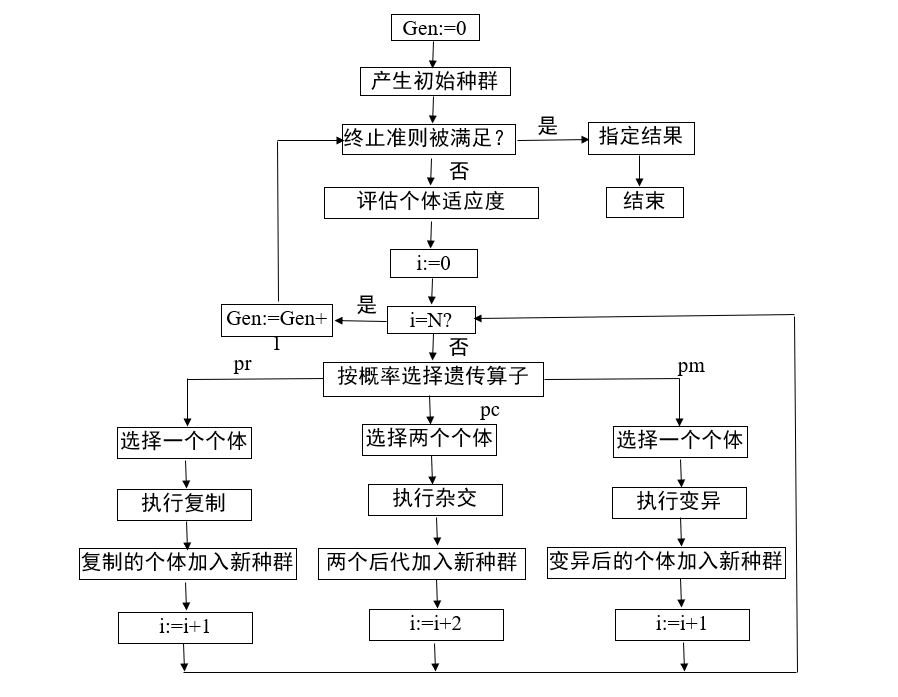
\includegraphics[scale=0.4]{../images/GP_framework.png}
\caption{遗传程序设计的流程图}
\label{fig:label}
\end{figure}
}

\frame{\frametitle{算法}
遗传程序设计的基本算法:	
	
(1)随机生成初始群体,其中个体是由表示问题的函数和终止符随机组合而成的计算机程序。
	
(2)循环执行下列各步直到满足终止准则为止:

I)运行群体中的每个计算机程序,并对其赋予适应度;

II)运行下面两个主要操作产生新的计算机程序群体:

\qquad i)把当前一代计算机程序复制成新一代计算机程序,被复制的个体依其适应度随机选定。

\qquad ii)随机选定双亲个体部位进行交叉操作产生新个体,双亲个体也依适应度随机选定。

(3)用结果标定法确定的程序被认为是运行的结果,它可能是一个正确(或近似)的问题答案。
}

\frame{\frametitle{关键}
遗传程序设计所需解决的关键问题:	
	
(1)程序的表示;

(2)程序好坏的评价标准;

(3)遗传算子的设计。
}

\frame{\frametitle{程序的表示}	
\parindent=19pt	
\renewcommand{\raggedright}{\leftskip=0pt \rightskip=0pt plus 0cm}
\raggedright
在遗传程序设计中,种群中的个体是计算机程序。为了程序表示的简单性和容易验证程序的句法,遗传程序设计用LISP语言来表示程序。

考虑一个简单的LISP程序,该程序简单地返回一个自然数n的平方:
	
>(defun square(n)(*nn))

SQUARE

下面是一个计算实数绝对值的LISP程序:

>(defun abs(x)(if(< x 0)(-x)(x)))

ABS

LISP程序的主体由类似于(*nn)和(if(< x 0)(-x)(x))的一些S-表达式所组成。

一般来说一个表示LISP程序的S-表达式通常由一些函数和端点组成。
}

\frame{\frametitle{程序的表示}	
\parindent=19pt	
\renewcommand{\raggedright}{\leftskip=0pt \rightskip=0pt plus 0cm}
\raggedright
构造LISP程序的S-表达式是以前缀表达式形式表示的。给定一个S-表达式,我们容易构造出它的语法树,而对该树进行先序遍历便可得到给定的S-表达式。
	
例如S-表达式(+12(if(> x 10)56))所对应的语法树如下图所示:

	\begin{figure}[ht]
		\centering	
		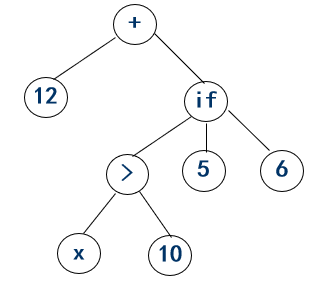
\includegraphics[scale=0.3]{../images/syntactic_tree.png}
		\caption{S-表达式的语法树}
		\label{fig:label}
	\end{figure}
	
在语法树中,树的外部结点(叶结点)分别用变量x和常量5,6,10,12来标记,这些变量和常量通常称为端点,而内部结点分别用函数+,>,IF来标记。
}

\frame{\frametitle{实现}
用遗传程序设计求解问题有以下五个基本步骤:
	\begin{itemize}		
		\item<1-> 选择端点集;
		\item<2-> 选择函数集;
		\item<3-> 确定适应函数;
		\item<4-> 确定控制参数;
		\item<5-> 确定指定结果的方法和终止程序运行的条件。
	\end{itemize}
}

\frame{\frametitle{选择端点集和函数集}
\renewcommand{\raggedright}{\leftskip=0pt \rightskip=0pt plus 0cm}
\raggedright
	\begin{itemize}		
		\item<1-> 在遗传程序设计中,计算机程序用LISP程序的语法树来表示。每一棵语法树的内部结点由一些函数构成,而叶结点由一些变量和常数构成。
		\item<2-> 对于一个给定的问题,首先要确定由所有可能求解该问题的程序所组成的程序空间S。由于LISP程序通常可以由一些简单的函数、变量和常数经过有限次运算和复合而生成。因此若要指定程序空间S,我们只要指定可以构成中程序的函数集和端点集。
		\item<3-> 函数集可以包含:
		
			<1> 算数运算 +,-,*,/等;
			
			<2> 数学函数 sin,cos,exp,log等;
			
			<3> 布尔运算 AND,OR,NOT等;
			
			<4> 条件运算 IF-THEN-ELSE等;
			
			<5> 循环运算 DO-UNTIL,FOR,WHILE等。
		\item<4-> 端点集通常由变量和常量组成。
	\end{itemize}
}

\frame{\frametitle{初始化}
	\renewcommand{\raggedright}{\leftskip=0pt \rightskip=0pt plus 0cm}
	\raggedright
	\begin{itemize}		
		\item<1-> 假设问题的端点集和函数集分别为T和F。
		\item<2-> 初始种群中的每个S-表达式,即每棵树,可按以下步骤产生:
		
			<1> 首先建立一个根结点,从函数集F中随机地选择一个函数作为根结点的标记;
		
			<2> 每当树中的一个结点被标记为函数集F中的一个函数f后,则为该结点建立z(f)个儿子结点,而每个儿子结点的标记从C=FYT中随机地选取;
		
			<3> 每当树中一个结点被标记为端点集T中的一个元素时,则该结点成为树的一个叶结点;
		
			<4> 如此反复进行,直到所有结点都被标记。
	\end{itemize}
}

\frame{\frametitle{初始化}
	\renewcommand{\raggedright}{\leftskip=0pt \rightskip=0pt plus 0cm}
	\raggedright
	\begin{itemize}		
		\item<1-> 假定F=\{+,-,*,/\},T=\{a,b,c,d\}。下面给出了建立一棵树结构的过程:
			\begin{figure}[ht]
			\centering	
			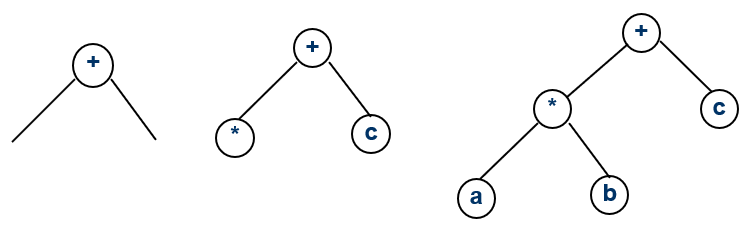
\includegraphics[scale=0.3]{../images/build_tree.png}
			\caption{语法树的构建}
			\label{fig:label}
			\end{figure}
		\item<2->上述树生成过程可以有几种不同的实现方式:
		
			<1> 完全法:该方法预先定义所要生成的树的最大深度Di,当要生成的结点的深度小于最大深度时,则从函数集F中随机地选取一个元素作为该结点的标记,当要生成的结点的深度等于最大深度时,则从端点集T中随机地选取一个元素作为该结点的标记。
	\end{itemize}
}

\frame{\frametitle{初始化}
	\renewcommand{\raggedright}{\leftskip=0pt \rightskip=0pt plus 0cm}
	\raggedright	
	<2> 生长法:该方法预先定义所要生成的树的最大深度Di,当要生成的结点的深度小于最大深度时,则从    中随机地选取一个元素作为该结点的标记,当要生成的结点的深度等于最大深度时,则从端点集T中随机地选取一个元素作为该结点的标记。
	
	<3> 混合法:该方法预先定义所要生成的树的最大深度Di,对从2至最大深度的每一个深度,生成相同个数的树。对每一个深度,其中一半的树用完全法生成,而另一半用生成方法生成。

	\parindent=19pt		
	例如,假定树的最大深度定义为6,种群中个体的个数为100,则用混合方法将分别产生深度为2,3,4,5,6的树各20个,其中深度为的树有10个用完全法产生,有10个用生成方法产生。
}

\frame{\frametitle{适应函数}
	\parindent=19pt	
	\renewcommand{\raggedright}{\leftskip=0pt \rightskip=0pt plus 0cm}
	\raggedright
	适应性函数是遗传算法和遗传程序设计得以实现的关键因素,是评价个体好坏的定量表述,决定着演化过程中群体选择复制及群体整体性的质量。

	与其它演化算法相同,在遗传程序设计中,个体的适应性函数值是判断个体的质量的唯一办法。
	
	个体适应性函数值的计算方法是问题相关的,有多种方式度量个体的适应性函数值,有些方法是明确的,有些方法是隐含的。
	
	例如,若个体是下列程序:
		\begin{figure}[ht]
		\centering	
		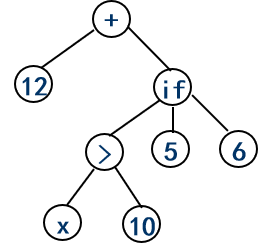
\includegraphics[scale=0.3]{../images/program.png}
		\caption{程序示例}
		\label{fig:label}
		\end{figure}
}

\frame{\frametitle{适应函数}
	\renewcommand{\raggedright}{\leftskip=0pt \rightskip=0pt plus 0cm}
	\raggedright
	评估该程序好坏的一种方法是:
	
	(1) 建立一个样本集$\{(x_{i},y_{i})|i=1,2,\Lambda,s\}$,其中$y_{i}$是当变量x取值为$x_{i}$时的期望输出;

	(2) 当$x=x_{i}(i=1,2,\Lambda,s)$时,运行该程序得到输出$z_{i}$;

     (3) 计算所得到的输出与期望输出之间的误差的绝对值之和$e=\Sigma|z_{i}-y_{i}|$;

     (4) 最后,用e作为该个体的适应性函数值。显然,适应性函数值越小,个体越好。
	
	\parindent=19pt	
	若个体是判定树,则判定树的分类准确率可以作为个体的适应性函数值。若个体是游戏策略,则游戏策略与其它策略对奕时取胜的次数可以作为个体的适应性函数值。
}

\frame{\frametitle{适应函数}
	\renewcommand{\raggedright}{\leftskip=0pt \rightskip=0pt plus 0cm}
	\raggedright
	个体适应性函数值有以下几种形式:
	
	(1) 原始适应性函数值;
	
     原始适应性函数值是以问题本身的自然术语叙述的适应性函数值度量。

     (2) 标准适应性函数值;
	
     标准适应性函数值对原始适应性函数值作简单变换,使得标准适应性函数值越小,个体越好。

     (3) 调整适应性函数值;

     调整适应性函数值$\epsilon(0,1]$。调整适应性函数值越大,个体越好。

     (4) 正规化适应性函数值。
		
	\parindent=19pt	
	正规化适应性函数值$\epsilon[0,1]$,在基于适应性函数值比例的选择策略中可直接用作选择概率。
}

\frame{\frametitle{适应函数}
	\renewcommand{\raggedright}{\leftskip=0pt \rightskip=0pt plus 0cm}
	\raggedright
	设计适应性函数,一般有以下几个步骤:
	
	(1) 原始适应性函数;
	
     按照目标函数的计算方法直接计算原始适应性函数值。

     (2) 标准化适应性函数;
	
     将得出的原始适应性函数表述为标准适应性函数。

     (3) 优化调整适应性函数;

     调整最优个体与次优个体的微小差别。

     (4) 正规化适应性函数。
		
	正规化(归一化)已优化调整的适应性函数值。
}

\frame{\frametitle{父体选择策略}
	\renewcommand{\raggedright}{\leftskip=0pt \rightskip=0pt plus 0cm}
	\raggedright	
	(1) 通常,遗传程序设计使用基于适应性函数值比例的选择策略。
	
	(2) 若种群规模在1000以上,则经常使用一种贪婪过度选择策略。
	
	(3)该策略首先将种群中的个体按适应性函数值排序,然后将种群中的个体分为两部分。第一部分包含种群$x\%$的最好个体,另一部分包含其它$(1-x\%)$的个体。当进行父体选择时,80\%的选择在第一部分中进行,20\%的选择在第二部分中进行。x的取值以来于种群规模,通常通过实验确定。
		\begin{figure}[ht]
			\centering	
			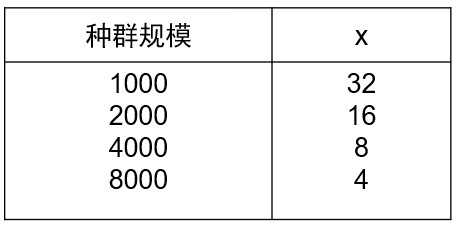
\includegraphics[scale=0.3]{../images/x_value.png}
			\caption{x的取值}
			\label{fig:label}
		\end{figure}
	
	\parindent=19pt	
	从上表可以看出,随着种群规模的增加,x不断减小,选择压力逐步增大。
}

\frame{\frametitle{遗传算子}
	\parindent=19pt
	\renewcommand{\raggedright}{\leftskip=0pt \rightskip=0pt plus 0cm}
	\raggedright	
	遗传程序设计中的遗传算子主要有复制、杂交和变异。变异算子的作用不及遗传算法中重要。
	
	(1) 复制
	
	复制算子首先按照某种基于适应性函数值比例的选择策略从种群中选择一个个体,然后将该个体不加改变地复制到下一代种群。

    复制算子有一个参数$p_{r}$,通常取$p_{r}=0.1$。
	
	(2) 杂交

    杂交算子分别从两个父体中随机地选择一个杂交点,然后交换父体中以杂交点为根结点的子树产生两个后代。
        \begin{figure}[ht]
			\centering	
			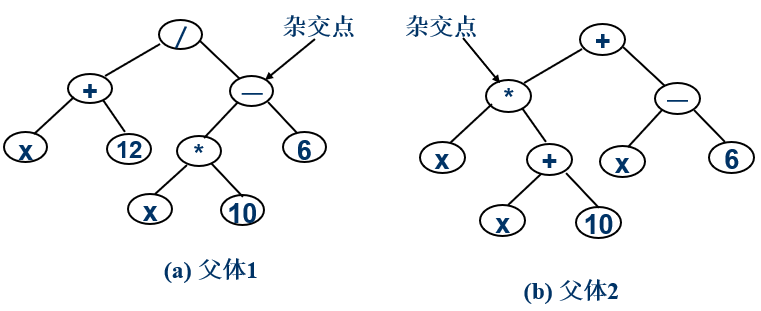
\includegraphics[scale=0.25]{../images/Hybridization1.png}
			\caption{x的取值}
			\label{fig:label}
		\end{figure}
}

\frame{\frametitle{遗传算子}
	\renewcommand{\raggedright}{\leftskip=0pt \rightskip=0pt plus 0cm}
	\raggedright	
        \begin{figure}[ht]
			\centering	
			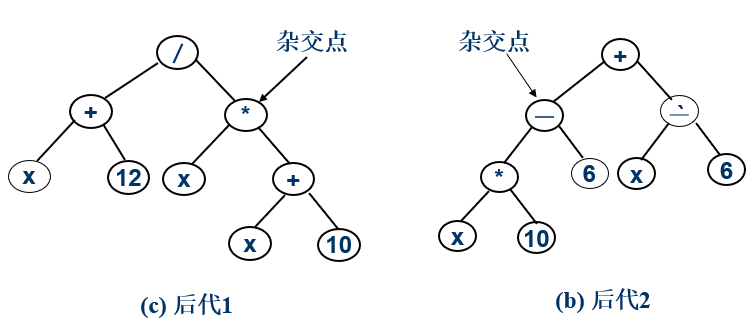
\includegraphics[scale=0.25]{../images/Hybridization2.png}
			\caption{x的取值}
			\label{fig:label}
		\end{figure}

    \parindent=19pt	
    杂交算子有两个参数 $p_{c}$和$p_{cn}$,$p_{c}$是按概率选择遗传算子时选择杂交算子的概率,而$p_{cn}$是在进行杂交时,在父体中选择内结点作为杂交点的概率。通常取$p_{c}=0.9$和$p_{cn}=0.9$。

    在对父体进行杂交后,后代树的深度有可能加大。为了有效地利用计算机资源,防止产生巨型个体,遗传程序设计通常设置一个最大允许深度  $D_{c}$进行控制。

    若杂交后,有一个后代的深度超过了最大允许深度,则随机地选取一个父体代替该后代;若两个后代的深度都超过了最大允许深度,则用两个父体代替这两个后代。
}

\frame{\frametitle{遗传算子}
    \renewcommand{\raggedright}{\leftskip=0pt \rightskip=0pt plus 0cm}
	\raggedright	
    (3) 变异
    
    \parindent=19pt
    变异算子首先在父体中随机地选择一个结点,然后删除以该结点为根结点的子树,并在该结点处插入一个随机生成的子树。
        \begin{figure}[ht]
			\centering	
			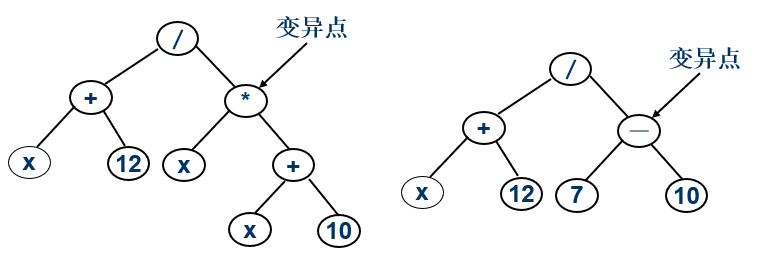
\includegraphics[scale=0.25]{../images/variation.png}
			\caption{x的取值}
			\label{fig:label}
		\end{figure}
	
	变异算子有两个参数$p_{m}$和$p_{mm}$。$p_{m}$是按概率选择遗传算子时选择变异算子的概率,而$p_{mm}$是在进行变异时,在父体中选择内结点的概率。
	
	值得注意的是J.R.Koza建议$p_{m}$,也就是说在遗传程序设计中不使用变异算子。近年来的遗传程序设计实践建议使用变异算子,但是以较低的概率。
	
}

\frame{\frametitle{应用}
	\begin{itemize}
		\item<1-> 预测和分类:使用历史数据库来预测新事例。
		\item<2-> 符号压缩:发现各变量间的隐含关系。
		\item<3-> 机器人:控制机器人行为,使其对环境做出反应。
		\item<4-> 人工生命:用计算机模拟生物的自然进化或发现规律。
		\item<5-> 神经网络设计“设计神经网络结构、发现学习规则和相关权值,以使神经网络完成指定的任务。
		\item<6-> 图像和信号处理:图像识别、图像恢复、图像和声音的压缩等。
		\item<7-> 多Agent系统的自动设计:多个Agent协作共同处理实际问题。
		\item<8-> 游戏策略:发现一个策略打败对手。
		\item<9-> 艺术:声音、三维图像的生成、计算机动画等。
	\end{itemize}
}

\frame{\frametitle{应用实例1}
	\renewcommand{\raggedright}{\leftskip=0pt \rightskip=0pt plus 0cm}
	\raggedright	
	\begin{figure}[ht]
	\centering	
	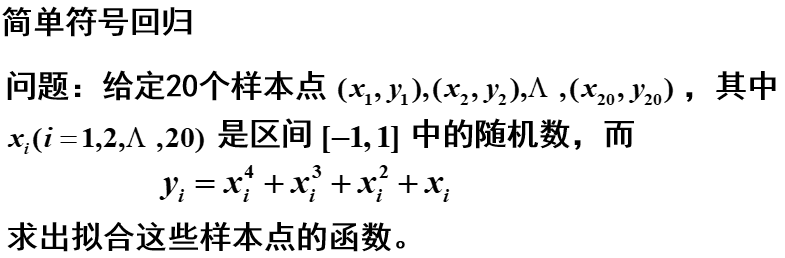
\includegraphics[scale=0.5]{../images/question.png}
	\end{figure}
}

\frame{\frametitle{应用实例1}
	\renewcommand{\raggedright}{\leftskip=0pt \rightskip=0pt plus 0cm}
	\raggedright	
	\begin{figure}[ht]
		\centering	
		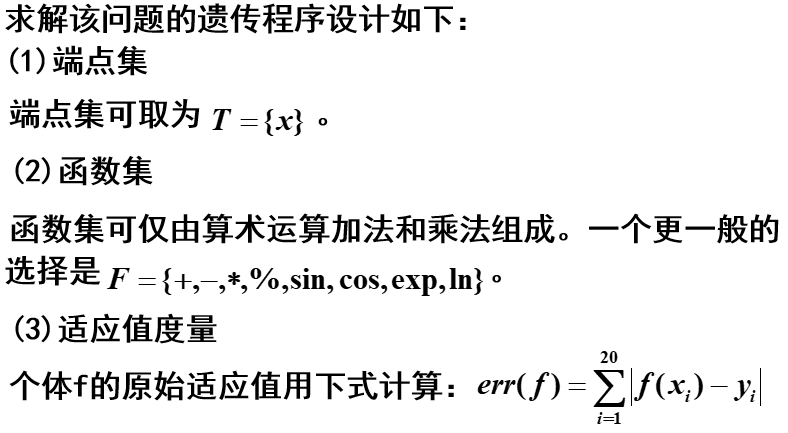
\includegraphics[scale=0.5]{../images/answer1.png}
	\end{figure}
}

\frame{\frametitle{应用实例1}
	\renewcommand{\raggedright}{\leftskip=0pt \rightskip=0pt plus 0cm}
	\raggedright	
	\begin{figure}[ht]
		\centering	
		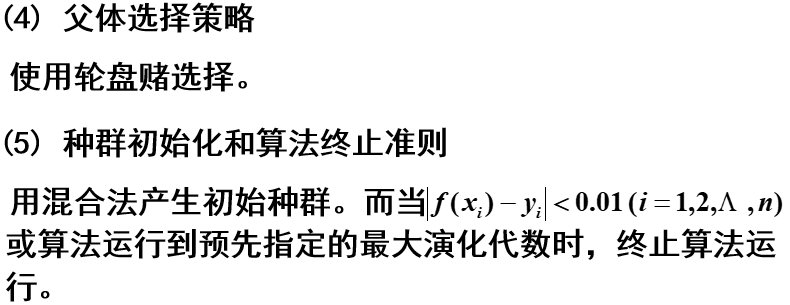
\includegraphics[scale=0.5]{../images/answer2.png}
	\end{figure}
}

\frame{\frametitle{应用实例1}
	\renewcommand{\raggedright}{\leftskip=0pt \rightskip=0pt plus 0cm}
	\raggedright	
	\begin{figure}[ht]
		\centering	
		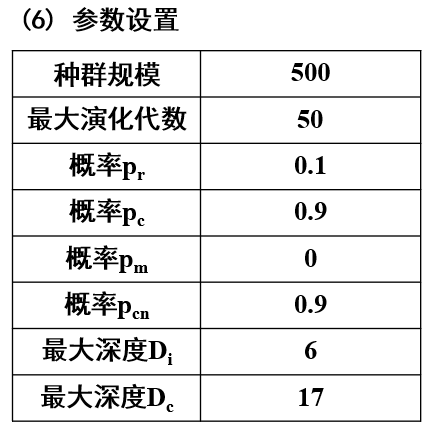
\includegraphics[scale=0.5]{../images/answer3.png}
	\end{figure}
}

\frame{\frametitle{应用实例1}
	\renewcommand{\raggedright}{\leftskip=0pt \rightskip=0pt plus 0cm}
	\raggedright	
	\begin{figure}[ht]
		\centering	
		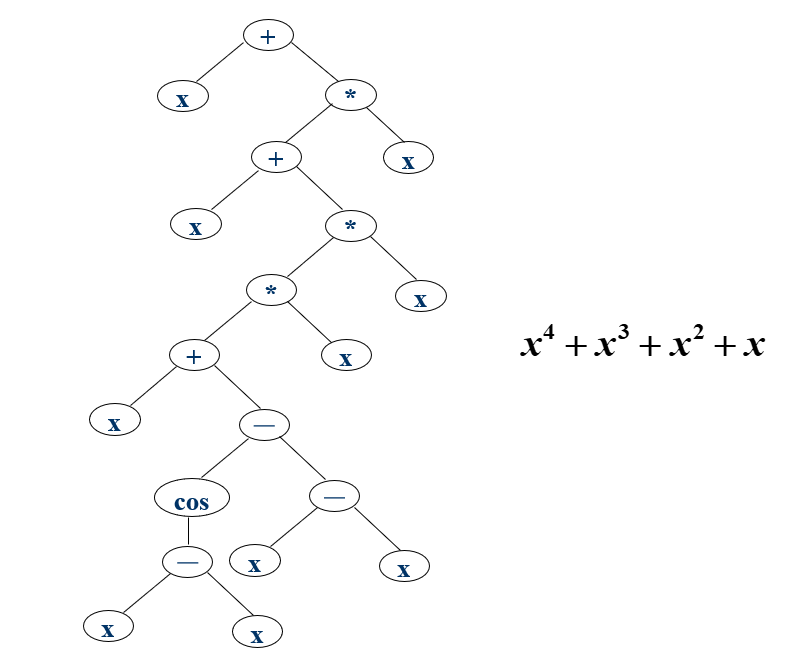
\includegraphics[scale=0.45]{../images/answer4.png}
	\end{figure}
}

\frame{\frametitle{应用实例2}
	\parindent=19pt
	\renewcommand{\raggedright}{\leftskip=0pt \rightskip=0pt plus 0cm}
	\raggedright	
	问题:给定数学表达式cos(2x),我们希望发现与cos(2x)恒等的数学表达式。
	
	将该问题视为一个符号回归问题。通过在某个区间内抽取一个随机样本,并计算给定函数在该样本的函数值,这样形成一组样本点,对所形成的样本点作符号回归。
}

\frame{\frametitle{应用实例2}
	\renewcommand{\raggedright}{\leftskip=0pt \rightskip=0pt plus 0cm}
	\raggedright	
	\begin{figure}[ht]
		\centering	
		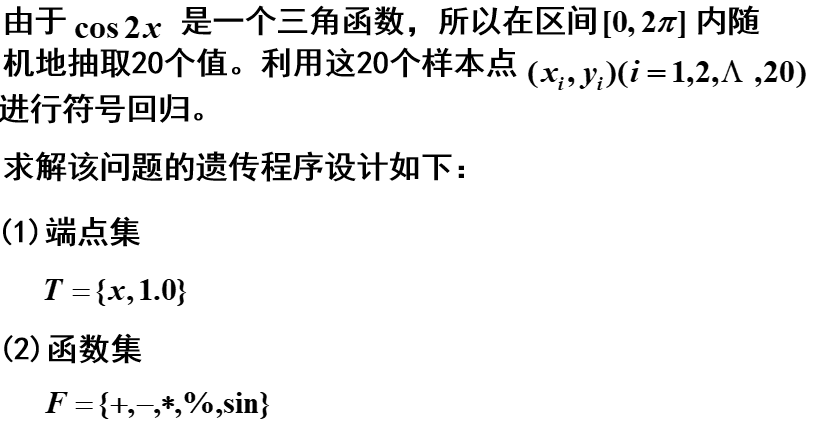
\includegraphics[scale=0.5]{../images/answer11.png}
	\end{figure}
}

\frame{\frametitle{应用实例2}
	\renewcommand{\raggedright}{\leftskip=0pt \rightskip=0pt plus 0cm}
	\raggedright	
	\begin{figure}[ht]
		\centering	
		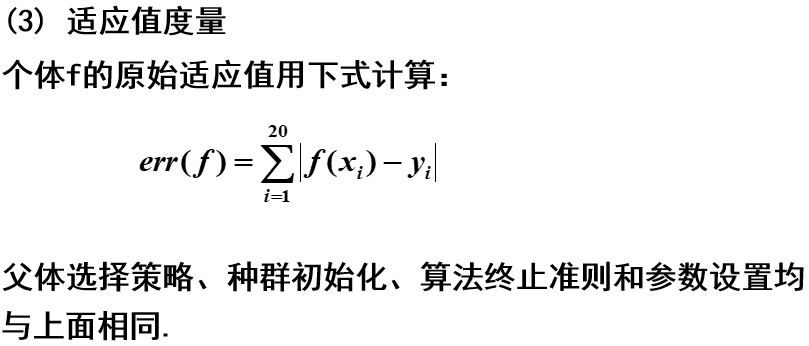
\includegraphics[scale=0.5]{../images/answer22.png}
	\end{figure}
}

\frame{\frametitle{应用实例2}
	\renewcommand{\raggedright}{\leftskip=0pt \rightskip=0pt plus 0cm}
	\raggedright	
	\begin{figure}[ht]
		\centering	
		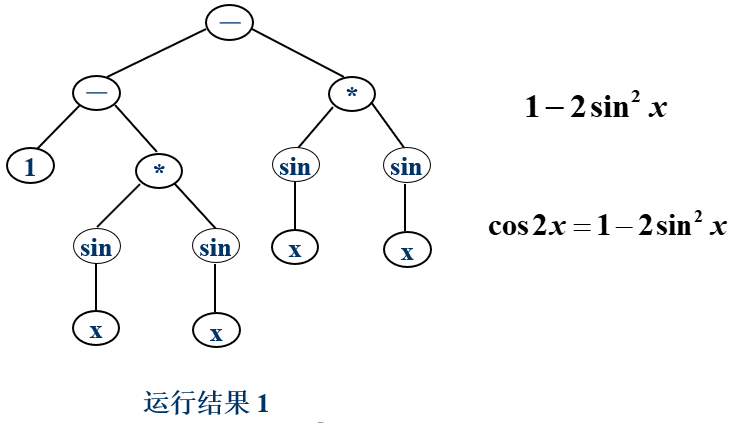
\includegraphics[scale=0.5]{../images/answer33.png}
	\end{figure}
}

\frame{\frametitle{应用实例2}
	\renewcommand{\raggedright}{\leftskip=0pt \rightskip=0pt plus 0cm}
	\raggedright	
	\begin{figure}[ht]
		\centering	
		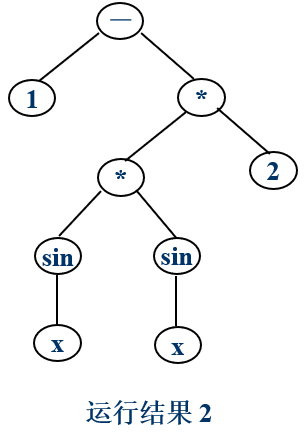
\includegraphics[scale=0.5]{../images/answer44.png}
	\end{figure}
}

\frame{\frametitle{应用实例2}
	\renewcommand{\raggedright}{\leftskip=0pt \rightskip=0pt plus 0cm}
	\raggedright	
	\begin{figure}[ht]
		\centering	
		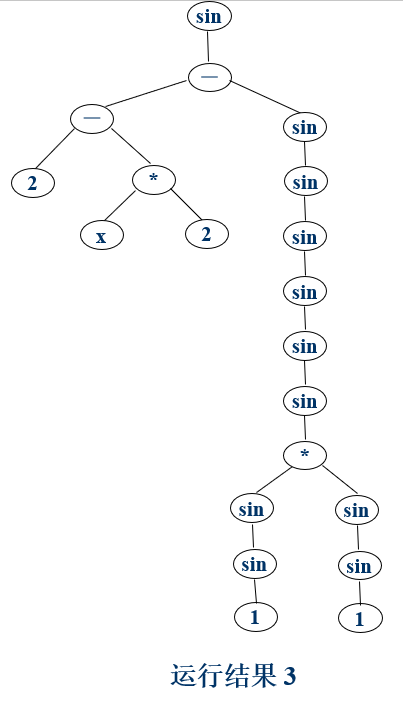
\includegraphics[scale=0.45]{../images/answer55.png}
	\end{figure}
}

\frame{\frametitle{应用实例2}
	\renewcommand{\raggedright}{\leftskip=0pt \rightskip=0pt plus 0cm}
	\raggedright	
	\begin{figure}[ht]
		\centering	
		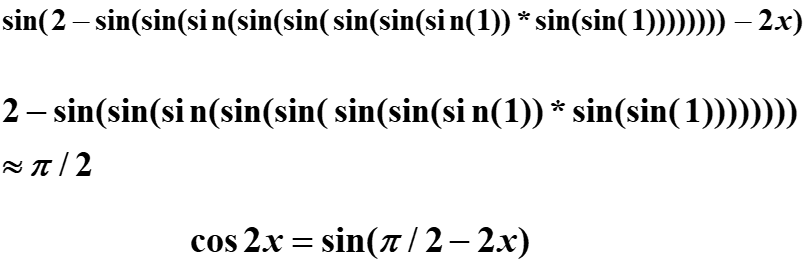
\includegraphics[scale=0.5]{../images/answer66.png}
	\end{figure}
}

\frame{\frametitle{改进}
	\parindent=19pt	
	\renewcommand{\raggedright}{\leftskip=0pt \rightskip=0pt plus 0cm}
	\raggedright
	遗传程序设计作为一种优化算法具有不需要先验性假设而可以进行全局搜索和进化最终得到最优解的特点,近年来人们在研究使用这种算法的过程中,也针对实际应用对其作了一些相应的改进。
	
	遗传程序设计主要处理树状具有分层结构的程序,在实际编程中多采用LISP语言实现。LISP语言由于缺乏统一的标准和方便的对外接口,作为一种解释语言运行速度较慢,可以采用几种具有不同数据类型的语言如PROL0G和C语言来加速程序进化的进程。
	
	传统的遗传程序设计限制少、搜索速度慢,可以用定向的非周期图(DAG)取代树和森林存储程序群体,针对子树进行改进,以节省程序的运行时间和空间。
	
	在算法方面,遗传程序设计可以与包括遗传算法、神经网络和模拟退火等的其他优化方法相结合,以得到更好的应用。
}

%end
